\chapter{RADIUS}
In contesti reali dove le reti hanno una dimensione molto elevata, usare un sistema di autenticazione CHAP-like come visto fino ad ora è impensabile. Questo p erché esistono diversi modi di connettersi alla rete e quando i numeri sono grandi possiamo riscontrare tre problemi principali:
\begin{itemize}
    \item Se mantengo DB distribuiti ci sono tanti punti che possono essere attaccati.
    \item Quando viene cambiato il valore di una variabile (es. una password) bisogna propagare l'informazione a tutti i DB.
    \item C'è necessità di avere \textit{qualcuno} dotato di permessi di gestione (admin).
\end{itemize}
Per questo è stato sviluppato RADIUS, che sfrutta dei \textbf{server (logicamente) centralizzati}, mantenendo \textbf{1 server primario} più altri server secondari replicati.
\section{Funzionamento e Autenticazione}
\begin{definition}[RADIUS - Remote Authentication Dial In User Service]
Protocollo di tipo \textbf{AAA UDP-based}\footnotemark, che fornisce: 
\footnotetext{\textsuperscript{\thefootnote}Triple A}
\begin{itemize}
    \item \textbf{(Remote) Authentication:} certifica l'identità digitale di un utente, anche se questo non può connettersi alla stessa rete del server autenticante.
    \item \textbf{Authorization:} gestisce i \textbf{permessi} di \textbf{accesso} ai servizi degli utenti autenticati.\footnotemark
    \footnotetext{\textsuperscript{\thefootnote}ES: un set di canali di una pay-per-view che rientrano nell'abbonamento dell'utente.}
    \item \textbf{Accounting:} \textbf{tiene traccia} delle \textbf{azioni eseguite dagli utenti}\footnotemark
    \footnotetext{\textsuperscript{\thefootnote}ES: quando tempo passano su un servizio X o la spesa fatta per un bene Y.}
\end{itemize}
\end{definition}
\begin{figure}[h]
    \centering
    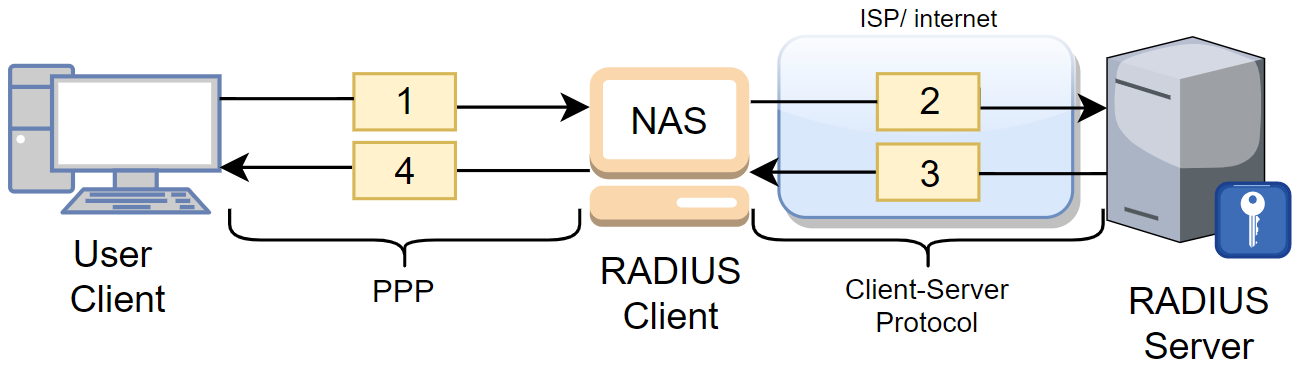
\includegraphics[width=0.8\textwidth]{image/radius.png}
    \caption{Main RADIUS components}
    \label{fig:radiusscheme}
\end{figure}\pagebreak
Le principali componenti del protocollo sono le seguenti:
\begin{definition}[RADIUS Entities]
\begin{itemize}
    \item \textbf{PPP} (Point to Point Protocol): Utilizzato per l'autenticazione tra il sistema dell'utente ed il \textbf{NAS/RAD client}. Generalmente si usano PAP o CHAP.
    \item \textbf{RADIUS Client/NAS} (Network Access Server): \textit{punto di accesso} che permette agli utenti di autenticarsi nella rete per sfruttarne i servizi. 
    \item \textbf{RADIUS Server:} \textbf{mantengono} le \textbf{credenziali degli utenti} in DB centralizzati ed erogano i servizi offerti dalla rete. I database sono di tre tipi:
    \begin{itemize}
        \item \textbf{Registered User Database:} per ogni utente si mantengono le credenziali e le modalità di autenticazione e gli attributi relativi al servizio di autorizzazione.
        \item \textbf{Client Database:} Mantiene le informazioni relative ai \textit{NAS} ammessi come radius client. 
        \item \textbf{Accounting Database:} Per ogni utente vengono mantenute informazioni relative al servizio di accounting.
    \end{itemize}
\end{itemize}
\end{definition}
Il processo di autenticazione avviene (nei minimi dettagli) nel seguente modo: 
\begin{proposition}[RADIUS Authentication \cref{fig:radiusscheme}]
\begin{enumerate}
    \item \textbf{PPP Request:} l'\textbf{utente invia} le proprie credenziali al \textbf{RAD client}.
    \item \textbf{RADIUS Request:} il NAS converte/include le credenziali ricevute in un \textbf{Messaggio di Richiesta}, che invia al \textbf{RAD Server}
    \item \textbf{RADIUS Response:} il \textbf{RAD Server} elabora la richiesta e produce un \textbf{Messaggio di Risposta}, che invia al \textbf{RAD client} che l'aveva contattato.
    \item \textbf{PPP Response:} il NAS notifica all'utente l'esito dell'autenticazione ricevuto dal server.
\end{enumerate}
\end{proposition}
\subsection{Servizio di Proxy}
Il protocollo RADIUS supporta connessioni remote, anche quando non possiamo connetterci direttamente alla rete desiderata. Difatti i RADIUS server svolgono la funzione di \textbf{Proxy Server} per altri RADIUS server \textbf{remoti}.
\begin{theorem}[Servizio di Proxy]
 Eseguono i servizi per conto di altri RADIUS server (es. facendo \textit{roaming} tra diversi ISP). Le funzionalità di proxy possono essere svolte sia in maniera trasparente che non, specificandolo nel contenuto del messaggio.
\end{theorem}\pagebreak
\section{Pacchetti RADIUS}
Come ogni protocollo, RADIUS impone una precisa specifica per il formato dei suoi messaggi:
\begin{figure}[h]
    \centering
    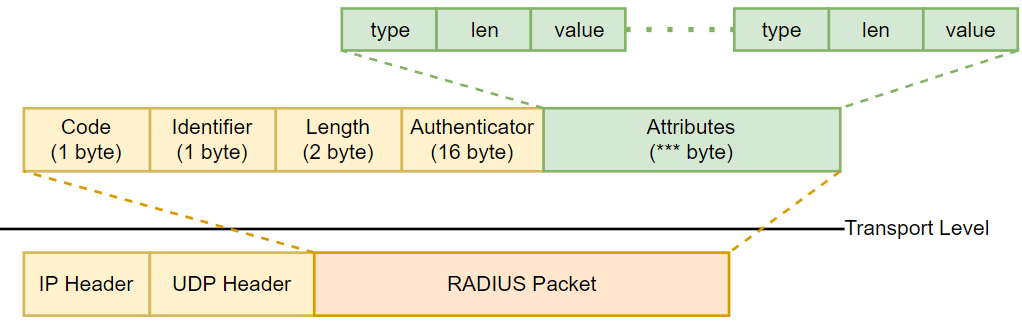
\includegraphics{image/radpack.png}
    \caption{RADIUS Packet Structure}
    \label{fig:radpack}
\end{figure}
\begin{itemize}
    \item \textbf{Code:} indica il \textbf{tipo} di \textbf{Pacchetto RADIUS}. I principali sono:
\end{itemize}
        \begin{definition}[Main Code Values]
        \begin{itemize}
            \item \textbf{Access-Request (1):} richiesta di autenticazione.
            \item \textbf{Access-Accept (2):} autenticazione avvenuta con successo.
            \item \textbf{Access-Reject (3):} autenticazione fallita/ rifiutata.
            \item \textbf{Accounting-Request (4):} richiesta di memorizzazione informazioni.
            \item \textbf{Accounting-Response (5):} risposta alla memorizzazione di informazioni.
            \item \textbf{Access-Challenge (11):} l'autenticazione richiede ulteriori messaggi.
        \end{itemize}
        \end{definition}
\begin{itemize}
    \item \textbf{ID:} specifica l'identificatore per l'autenticazione e serve a \textbf{legare} richiesta e risposta.
    \item \textbf{Length:} specifica la lunghezza del pacchetto, che è \textbf{sempre} compresa tra 20 e 4096 bytes.
    \item \textbf{Authenticator:} dipende dal tipo di pacchetto. Può essere:
    \begin{itemize}
        \item \textbf{Request:} \textbf{nonce} generata casualmente per il protocollo di autenticazione.
        \item \textbf{Response:} \textbf{digest MD5} per l'autenticazione del messaggio di risposta.
    \end{itemize}
    \item \textbf{Attributes:} lista di \textbf{campi} in formato \textbf{AVP} (Attribute Value Pair). Ogni campo è costituito da:
    \begin{itemize}
        \item \textbf{Type:} (1 byte) indica il tipo/significato del campo.
        \item \textbf{len:} lunghezza in byte del campo.
        \item \textbf{Value:} payload del campo.
    \end{itemize}
\end{itemize}
\begin{note}
Il campo attributes è un \textbf{extensible information field}.
\end{note}
\begin{definition}[Extensible Information Field]
Un campo è di tipo extensible information se il numero, il tipo e l'ordine delle informazioni contenute al suo interno può variare in base alle esigenze.
\end{definition}
\begin{remark}
Per costruzione non possiamo avere più di $2^8=256$ attributi differenti univocamente identificati a causa della dimensione del sottocampo \textbf{type}. In genere, un pacchetto di \textbf{Access-Request} contiene sempre i seguenti attributi:
\begin{itemize}
    \item \textbf{User-Name:} identificatore dell'utente.
    \item \textbf{User-Password:} password dell'utente, oscurata nel protocollo PPP-PAP.
    \item \textbf{Chap-Password:} challenge del protocollo PPP-CHAP, se utilizzato.
    \item \textbf{NAS-Identifier:} identificatore univoco del RADIUS client.
    \item \textbf{NAS-IP-Address:} indirizzo IP del RADIUS client.
    \item \textbf{NAS-Port:} porta UDP del RADIUS client.
\end{itemize}
\end{remark}

\section{Autenticazione in dettaglio}
Consideriamo il processo di autenticazione messo in atto dal RAD client e dal RAD server:
\begin{proposition}[Authentication Details]
\begin{enumerate}
    \item Il RAD client genera un \textbf{ID} per \textbf{identificare la richiesta} e una \textbf{nonce ReqAuth} per l'autenticazione. Mantiene la coppia \{\textbf{ID, ReqAuth}\} generata in un database locale ed invia una \textbf{RADIUS-Request}, contenente anche le credenziali di accesso ricevute tramite protocollo PPP dall'utente.
    \item Il RAD server genera una \textbf{RADIUS-Response}, composta da un digest prodotto tramite \textbf{MD5} secondo il seguente schema:
    \[\text{digest}=\text{MD5}(\text{Code||ID||Length||Auth||Attributes||S})\]
    \begin{itemize}
        \item \textbf{ID:} uguale per request e response.
        \item \textbf{Code, Length, Attributes:} specifiche del messaggio di risposta.
        \item \textbf{Auth:} nonce contenuta nel messaggio di richiesta e generata dal RAD Client.
        \item \textbf{S:} secret key condivisa tra RAD-client e RAD-server.
    \end{itemize}
    \item Il RAD-Client rigenera il digest utilizzando il suo DB per recuperare l'ReqAuth relativo all'ID ricevuto e verifica che sia uguale a quello ricevuto nella \textbf{RADIUS-Response}.
    \begin{itemize}
        \item In caso negativo, il RAD-Client comunica all'utente tramite protocollo PPP il fallimento dell'autenticazione. 
        \item In caso positivo, possiamo avere tre outcome diversi:
        \begin{enumerate}
            \item \textbf{response = Access-Accept:} viene comunicato all'utente tramite protocollo PPP l'avvenuta autenticazione e tutti i parametri di configurazione necessari.
            \item \textbf{response = Access-Reject:} le \textbf{credenziali di accesso} e/o degli \textbf{attributi nella richiesta} \textbf{non} sono \textbf{validi}. Viene comunicato all'utente il fallimento tramite protocollo PPP.
            \item \textbf{response = Access-Challenge:}Il RAD-Server ha bisogno di \textbf{ulteriori informazioni} per poter autenticare l'utente. Il \textbf{NAS} si occupa perciò di \textbf{recuperare} tali \textbf{informazioni} dall'utente ed invia una nuova \textbf{Access-Request.}
        \end{enumerate}
    \end{itemize}
\end{enumerate}
\end{proposition}
\begin{figure}[ht]
    \centering
    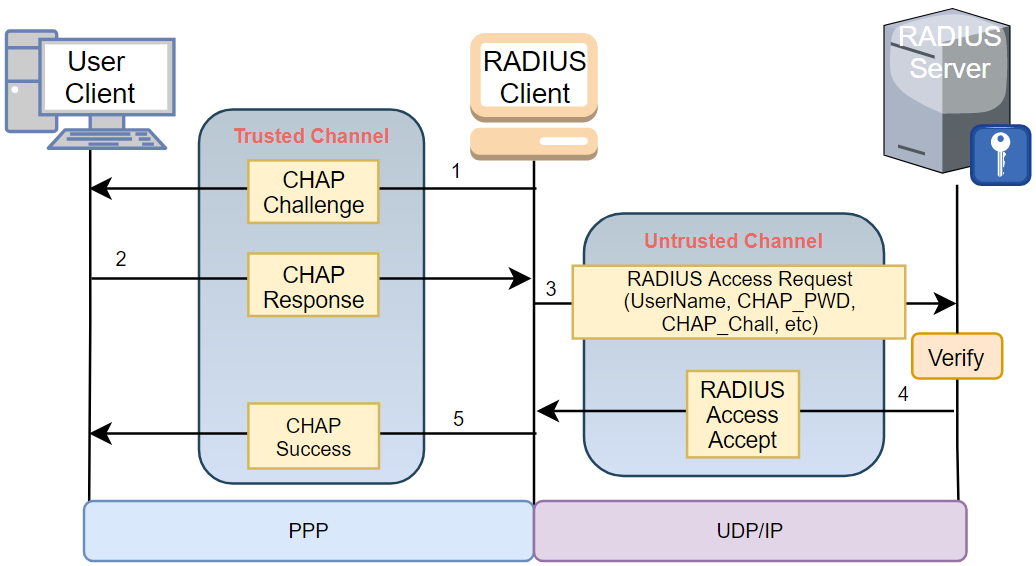
\includegraphics[width=0.85\textwidth]{image/chaprad.png}
    \caption{CHAP authentication in RADIUS}
    \label{fig:chaprad}
\end{figure}
\subsection{Challenge in PPP-CHAP}
Nel caso in cui PPP sia di tipo CHAP, la challenge per l'autenticazione CHAP tra utente e NAS viene gestita nel seguente modo:
\begin{definition}[PPP-CHAP]\label{def:chapradius}
\begin{enumerate}
    \item Il NAS genera la challenge per l'utente che vuole essere autenticato.
    \item L'utente genera ed invia ed invia la CHAP-response\footnotemark\, al RAD-client che la inoltrerà al RAD-Server insieme alla challenge.
    \item Il RAD-Server verifica la validità della coppia \{CHAP-challenge, CHAP-Response\} e di altri parametri tra cui l'ID, rigenerando la response tramite le credenziali in suo possesso e la challenge appena ricevuta.
\end{enumerate}
\footnotetext{\textsuperscript{\thefootnote}CHAP-Response $=$ H(user-PWD, CHAP-Challenge)}
\end{definition}
\section{Servizi di Sicurezza}
I servizi di sicurezza offerti dal protocollo sono: 
\begin{theorem}[Servizio di Sicurezza]
 \begin{itemize}
     \item \textbf{Autenticazione delle RAD Response:} i messaggi di risposta sono autenticati con un meccanismo \textbf{CHAP-Like}\footnotemark, basato sulla conoscenza di un segreto condiviso e sull'uso di una crypto-hash function.
     \item \textbf{Confidenzialità sulle PWD degli Utenti:} le password degli utenti sono criptate prima dell'autenticazione.
 \end{itemize}
 \footnotetext{\textsuperscript{\thefootnote}Viene evitato l'invio in chiaro delle password. In altre parole non c'è trasmissione di segreti.}
\end{theorem}
\subsection{Vulnerabilità nella Sicurezza}
I servizi di sicurezza offerti da RADIUS non sono perfetti, né lato autenticazione né su lato confidenzialità. Vediamo perché:
\begin{corollary}[Errori di Autenticazione]
\begin{itemize}
    \item Soltanto la \textbf{RADIUS Response} viene autenticata, lasciando spazio ad attacchi.
    \item Uso \textbf{forzato} della funzione hash \textbf{MD5} (non HMAC \cref{def:hmac})
    \item uso di \textbf{chiavi simmetriche} a \textbf{bassa entropia}.
\end{itemize}
\end{corollary}
\begin{corollary}
[Errori di Confidenzialità]
\begin{itemize}
    \item Meccanismi \textbf{personalizzati} per la cripatazione delle password.
    \item \textcolor{red}{\textbf{Riutilizzo della chiave di auth per fare encryption}}.
    \item Trasmissione in chiaro dei messaggi protocollari.
\end{itemize}
\end{corollary}
Osserviamo preliminarmente che la trasmissione in chiaro dei messaggi di request e response lascia spazio all'intercettazione di tali messaggi e, soprattutto, ad un eventuale modifica nel caso della request in quanto non autenticata.\\
Vediamo nel dettaglio cosa implicano queste debolezze:
\begin{proposition}[RADIUS Request Non Autenticata]
\begin{itemize}
    \item \textbf{Vulnerabilità a MITM:} data la mancanza di cifratura sul canale, i messaggi di request/response possono essere creati.
    \item \textbf{Payload Replay Attack:} Attacco su due fronti che permette di autenticarsi con l'identità dell'utente vittima.
    \begin{enumerate}
        \item Supponiamo di posizionarci tra il RAD-client e il RAD-server e di poter osservare un'autenticazione valida dell'utente, \textbf{salvando CHAP-Chappenge e CHAP-Response}. 
        \item L'attaccante avvia una nuova autenticazione a nome della vittima, utilizzando una password fasulla. Poiché il NAS non fa controllo ed inoltra la request verso il RAD-server, l'attaccante può intercettarla e sostituendo \textbf{CHAP-challenge} e \textbf{CHAP-response} precedentemente memorizzate \textbf{(coppia valida)} viene visto come utente legittimo.
    \end{enumerate}
\end{itemize}
\end{proposition}
\begin{theorem}[Soluzione con Message Authentication Extension Protocol]
Più che un protocollo vero e proprio è un container che specifica come un pacchetto di auth dovrebbe essere fatto. 
Tecnica utile per rendere il protocollo resistente ad attacchi MITM. Il funzionamento prevede l'\textbf{aggiunta} di un \textbf{nuovo attributo} nella Access-Request per il controllo dell'integrità.
\end{theorem}\pagebreak
Si hanno così due campi di autenticazione:
\begin{itemize}
    \item Uno nell'\textbf{header RADIUS}, costituito dalla nonce a 16byte per la richiesta di autenticazione.
    \item Uno negli \textbf{attributi}: MAC per il controllo di integrità della request calcolato come
    \[\text{MAC}=\text{HMAC-MD5(Code||ID||Length||Auth||Attributes||S)}\]
    Dove il valore dell'attributo \textbf{Authenticator} è zero in quanto lo si sta calcolando e verrà poi rimpiazzato
\end{itemize}
\subsection{Confidenzialità della password in PPP-PAP}
Nel caso in cui il protocollo PPP sia di tipo PAP, la password dell'utente nella RAD-Request viene criptata utilizzando una nonce data dall'\textbf{ReqAuth} e la chiave segreta \textbf{S}, così da non rivelarla ad eventuali attaccanti in ascolto. Il processo di cifratura delle passwrod è il seguente: 
\begin{definition}[PWD Encryption in RADIUS]
\begin{enumerate}
    \item Data la password si effettua un padding fino a 16 byte, questa è la dimensione del blocco.
    \item Si calcola la nonce di ReqAuth e si esegue MD5(S||ReqAuth). 
    \item La password prima di essere spedita viene cifrata calcolando 
    \[\text{PWD}\oplus\text{MD5(S||ReqAuth)}\]
\end{enumerate}
Se la password è più lunga di 16 byte, viene suddivisa in blocchi da 16 e l'ultimo blocco riempito con un padding. In quel caso, eseguiamo:
\begin{algorithmic}
\ForAll{$\text{PWD}_{\text{blk}}$}
\State $\text{PWD}_{\text{enc}}=\text{PWD}_{\text{blk}}\oplus\text{MD5(S||ReqAuth)}$
\EndFor
\end{algorithmic}
\end{definition}
\pagebreak
\begin{proposition}[Bassa entropia delle chiavi]
La bassa entropia è dovuta al basso numero di caratteri coinvolti nelle chiavi (viene usato il set ASCII). Inoltre, in molti casi, \textbf{una sola password è utilizzata per tutta la rete dell'ISP}. Gli attacchi possibili sono due:
\begin{itemize}
    \item \textbf{Dictionary Attack alla chiave segreta S in PPP-PAP:} E' possibile creare un dizionario di coppie \textbf{\{ReqAuth, MD5(S, ReqAuth)\}} ascoltando i messaggi di Access-Request. Poiché MD5 posiziona il segreto alla fine (\cref{sub:secretpos}), è possibile precalcolare come blocco singolo la prima parte del messaggio e fare bruteforce diventa facile.\\
    \begin{remark}
    In realtà non c'è neanche bisogno della coppia: Inviando una coppia \{(user-ID, user-PWD)\} arbitraria, il NAS può agire come fosse un oracolo in un attacco CPA. Infatti intercettando l'Access-Request inviata, possiamo fare ottenere un digest MD5 valido calcolando:
    \[\text{MD5(S, ReqAuth)}=\text{user-PWD attribute}\oplus\text{password}\]
    E adesso possiamo cifrare una password qualsiasi.
    \end{remark}
    \item \textbf{Attacco alle pwd degli utenti in PPP-PAP:} L'attaccante invia un user ID questa volta valido e una password arbitraria da 16 byte. Intercettando i messaggi di Access-Request possiamo produrre un digest MD5 valido calcolando:
    \[\text{MD5(S, ReqAuth)}=\text{user-PWD attribute}\oplus\text{password}\]
    Adesso l'attaccante può cifrare una password qualsiasi.
\end{itemize}
\end{proposition}
\begin{note}[Dictionary Attack to Shared Secret Details]\\
L'attacco bruteforce è possibile solo con pwd inferiori a 16byte. In particolare, il NAS stesso può essere usato come un oracle in un attacco CPA. Intercettando i messaggi di Access-Request otteniamo la user-password attribute (16 bytes) e il Request Authenticator (16 bytes). Facendo uno xor tra la password cifrata e quella in chiaro otteniamo il digest dell'MD5.
\end{note}
\begin{note}[User-PWD Attack Details]\\
Anche questo attacco funziona con password di 16 bytes. Una volta ottenuto il digest valido possiamo bypassare tutte le limitazioni imposte lato client, come il numero di tentativi valido di autenticazione al RADIUS server.
\end{note}
\begin{figure}[h]
    \centering
    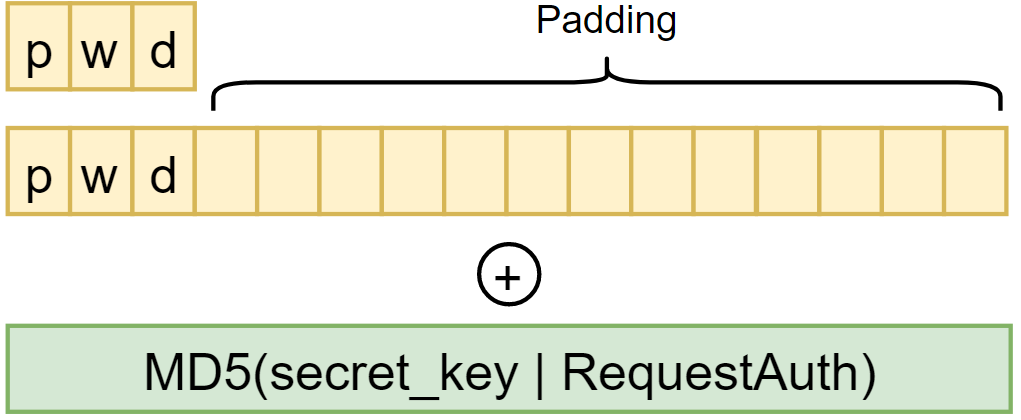
\includegraphics[width=0.5\textwidth]{image/radpwdenc.png}
    \caption{Password Encryption in RADIUS with PPP-PAP}
    \label{fig:radpwdenc}
\end{figure}
\subsection{Cattiva gestione dei PRNG}
Un'ulteriore errore commesso da RADIUS è una scarsa implementazione degli algoritmi di PRNG per la generazione delle nonce di ReqAuth, tipicamente non crypto-functions con \textbf{ciclo breve} (alta probabilità di collisione) e \textbf{alta predicibilità}. Questo significa che l'ipotesi di unicità della nonce viene meno e può permettere ad un attaccante di autenticarsi calcolando il valore della prossima nonce.\\
Ci sono 3 attacchi possibili che possono essere fatti:
\begin{itemize}
    \item \textbf{Birthday Attack:} Consideriamo un PRNG con ciclo di $2^n$ e al più $2^n$ valori differenti. Per il \textbf{paradosso del compleanno} \cref{eq:birthdayparadox} un valore si ripete con \textbf{probabilità del 50\%} con $2^\frac{n}{2}$ autenticazioni. Inoltre, alcune implementazioni potrebbero \textbf{usare più volte uno stesso PRNG} per generare una sola nonce, riducendo il ciclo di generazione.
    \item \textbf{Replay Attack:} L'attaccante può generare un dizionario \textbf{\{ID, AUTH, MD5\}} osservando coppie valide di \textbf{Access-Request/Access-Response} per effettuare un replay attack nel momento in cui il NAS genera una ReqAuth ripetuto. A quel punto è possibile autenticare/autorizzare un qualsiasi utente senza un pwd valida.\\
    L'ID può essere ricalcolato con brute-force in quanto costituito da un solo byte.
    \item \textbf{Attacco alle PWD degli utenti (se PPP-PAP):} Osservando le \textbf{Access-Request} l'attaccante genera un dizionario di \textbf{\{ReqAuth, PW-enc\}}. Se una nonce si ripete, è possibile ottenere informazioni sulle password degli utenti calcolando:
    \[\text{PW1}_{enc}\oplus\text{PW2}_{enc}=(\text{PW1}\oplus\text{MD5(S, ReqAuth)})\oplus(\text{PW2}\oplus\text{MD5(S, ReqAuth)})=\text{PW1}\oplus\text{PW2}\]
    Una volta ottenuto lo xor delle due passowrd in chiaro di due utenti bersaglio, poiché le dimensioni sono note e con buona probabilità di lunghezza differente, otteniamo in chiaro la parte finale della password più lunga e analizzando il risultato è possibile calcolare il risultato. Inoltre, è possibile velocizzare la generazione del dizionario effettuando delle Access-Request con password casuali (magari prese da un db online), consumando generazioni del PRNG.
\end{itemize}
\pagebreak
\section{DIAMETER}
RADIUS al giorno d'oggi è meno utilizzato di una volta in quanto presenta delle limitazioni importanti. In particolare:
\begin{itemize}
    \item \textbf{Scalabilità/Efficienza:} RADIUS supporta in maniera efficiente solo un numero ridotto di utenti. Questo è dovuto all'uso di UDP come protocollo di trasferimento, che implica un forte problema di packet loss nei casi di picchi di utenza.
    \item \textbf{Estensibilità:} il modo con cui gli attributi erano codificati imponeva limiti sulle nuove tecnologie e non era sufficiente a supportare possibili sviluppi futuri.
    \item \textbf{Interoperabilità:} non standardizzata e realizzata tramite soluzioni proprietarie (ogni venditore ha la sua soluzione).
\end{itemize}
DIAMETER è un'evoluzione di RADIUS, retrocompatibile e che risolve i le limitazioni analizzate prima. L'ottica con cui è sviluppato è simile alla logica "object-oriented": Viene definita una classe di \textbf{AAA Transport Profile} che specifica il tipo di livello di trasporto da usare (STCP/TCP-based) e una \textbf{base-class} DIAMETER più una serie di classi derivate per svariati tipi di servizi, tutte figlie della base-class.
\begin{note}
La DIAMETER Base Protocol è, più che un protocollo AAA, un protocollo di scambio di messaggi. 
\end{note}
\begin{figure}[h]
    \centering
    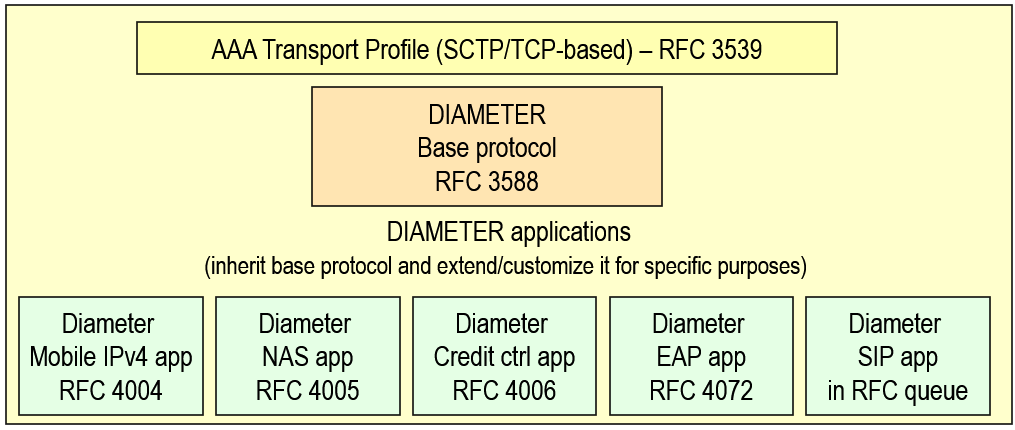
\includegraphics{image/diameter.png}
    \caption{DIAMETER Structure}
    \label{fig:diameter}
\end{figure}
\subsection{Feature Principali in DIAMETER}
\begin{proposition}[Trasporto Affidabile dei pacchetti]
 Utilizzo di \textbf{STCP/TCP} per il trasferimento affidabile dei pacchetti, instaurando connessioni persistenti tra client e server.
\end{proposition}
\begin{note}
    L'affidabilità è fondamentale per avere un accounting efficiente.
\end{note}
\begin{proposition}[Gestione degli Errori/Guasti standardizzata]
 L'error-control è demandato al livello applicativo. Inoltre, vengono implementate le seguenti funzionalità:
    \begin{itemize}
        \item \textbf{Rilevazione Duplicati:} vengono rilevati e scartati messaggi doppi.
        \item \textbf{Watchdog:} periodicamente vengono inviati dei pacchetti per conoscere lo stato dei vicini.
    \end{itemize}
\end{proposition}
\begin{note}
    In RADIUS la gestione degli errori dipende dall'implementazione
\end{note}
\begin{proposition}[Miglior Supporto all'Estensibilità]
il formato dei pacchetti è \textbf{modificato} e \textbf{ampliato}, per supportare più funzionalità. Tra i servizi implementati troviamo: 
    \begin{itemize}
         \item \textbf{Rilevazione Duplicati:} per ogni pacchetto vi è un ID.
        \item \textbf{Negoziazione:} è previsto un flag per specificare il comportamento che il destinatario deve attuare alla ricezione di parametri non supportati. 
    \end{itemize}
\end{proposition}
\begin{remark}
    RADIUS non supporta la rilevazione di duplicati né capacità di negoziazione dei parametri. Questo significa che il sistema non sa come rispondere ad un pacchetto con parametro non supportato.
\end{remark}
\begin{proposition}[Scoperta dei peers, configurazione e rilevamento capacità]
I \textbf{sistemi} DIAMETER \textbf{vicini} (peers) vengono \textbf{configurati} tramite \textbf{meccanismi automatici} accordandosi sulla versione del protocollo, sui meccanismi di sicurezza da usare e le applicazioni supportate.
\end{proposition}
\begin{proposition}[Supporto di Messaggi "Spontanei" da Server a Client]
Il server può inviare autonomamente dei messaggi al client al fine di supportare:
    \begin{itemize}
        \item \textbf{Disconnessioni volontarie} da parte del server.
        \item \textbf{Comunicazione di Errori/Fallimenti} al client.
        \item \textbf{Supportare} la \textbf{ri-autenticazione/ri-autorizzazione},
    \end{itemize}
\end{proposition}
    \begin{note}
    RADIUS supporta solo lo schema client-server, dove solo il primo avvia la comunicazione.
    \end{note}
\begin{proposition}[Gestione delle Entità Intermedie]
Viene specificata esplicitamente l'esistenza di diversi tipi di agenti, come \textbf{proxies, redirects, relay}. Inoltre, viene fatta distinzione tra:
    \begin{itemize}
        \item \textbf{Hop-By-Hop:} comunicazioni tra nodi intermedi.
        \item \textbf{End-To-End:} comunicazione tra nodi estremi, ovvero tra DIAMETER client e DIAMETER server.
    \end{itemize}
\end{proposition}
\begin{note}
    In RADIUS esiste solo hop-by-hop e non vengono specificate entità intermedie.
\end{note}
\subsection{Pacchetti DIAMETER}
I pacchetti DIAMETER possiedono il seguente formato:
\begin{itemize}
    \item \textbf{Header} [20 byte]: intestazione del messaggio
\end{itemize}
\begin{definition}[Header Structure]
\begin{itemize}
    \item \textbf{Version}[1byte]: versione del protocollo.
    \item \textbf{Message Length}[3 byte]: lunghezza del messaggio.
    \item \textbf{Flags}[1 byte]: flag per specificare la funzionalità
    \begin{itemize}
        \item \textbf{P (Request):} indica se il messaggio è una \textbf{richiesta}(1) o una \textbf{risposta} (0).
        \item \textbf{P (proxiable):} Indica se è possibile effettuare \textbf{proxying} del messaggio.
        \item \textbf{E (Error):} indica se è un messaggio di \textbf{errore}.
        \item \textbf{T:} indica se il messaggio è stato ritrasmesso.
    \end{itemize}
    \item \textbf{Command Code}[3 byte]: indica il \textbf{tipo} di messaggio.
    \item \textbf{Application ID}[4byte]: indica l'applicazione di appartenenza.
    \item \textbf{Hop-By-Hop ID}[4 byte]: identifica il canale tra due nodi intermedi della comunicazione.
    \item \textbf{End-To-End ID}[4 byte]: identifica gli estremi della comunicazione.
\end{itemize}
\end{definition}
\begin{figure}[h]
    \centering
    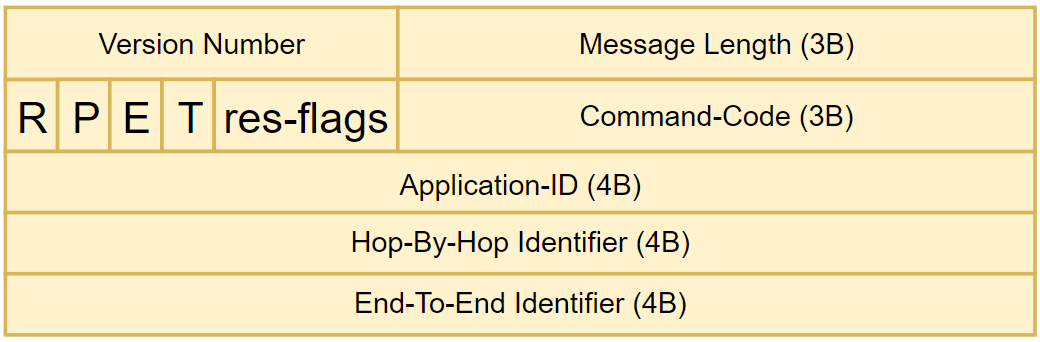
\includegraphics[width=0.7\textwidth]{image/diamheader.png}
    \caption{DIAMETER Header}
    \label{fig:diamheader}
\end{figure}
\begin{itemize}
    \item Attributes: Lista dei campi in formato \textbf{AVP}\footnotemark\,.
\end{itemize}
\begin{definition}[AVP format]
\begin{itemize}
    \item \textbf{AVP Code}[4 byte]: indica il tipo di campo.
    \item \textbf{Flags}[1 byte]: flag per indicare funzionalità.
    \begin{itemize}
        \item \textbf{V (Vendor):} indica se è presente il Vendor ID nell'AVP.
        \item \textbf{M (Mandatory):} indica se l'AVP deve essere \textbf{obbligatoriamente supportato}.
        \item \textbf{P (Protected):} Indica se è necessaria la criptazione end-to-end.
    \end{itemize}
    \item \textbf{AVP Length}[3 byte]: lunghezza del campo.
    \item \textbf{Vendor ID}[4 byte]: presente se \textbf{V=1}. Sostituisce il ruolo dell'AVP Code.
    \item \textbf{Data:} payload del campo.
\end{itemize}
\end{definition}
\footnotetext{Attribute Value Pair}
\begin{figure}[ht]
    \centering
    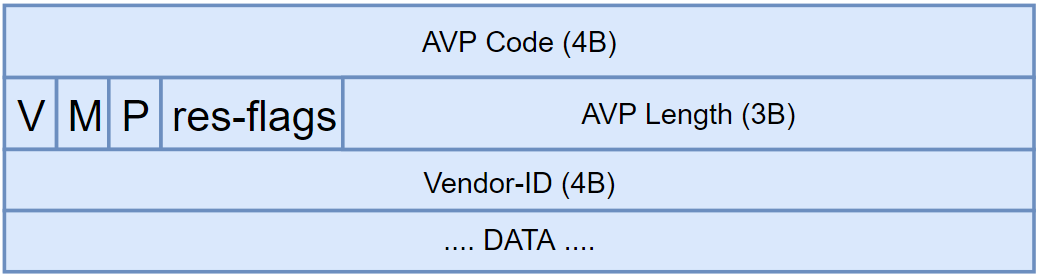
\includegraphics[width=0.7\textwidth]{image/avpheader.png}
    \caption{AVP Header}
    \label{fig:avpheader}
\end{figure}\pagebreak
\begin{note}\textbf{[Mandatory Flag-Bit]}\\
Questo flag negli AVP permette di realizzare il cosiddetto \textbf{Incremental Deployment}, ovvero la possibilità di implementare aggiornamenti nel sistema continuando a \textbf{supportare meccanismi preesistenti}. In particolare, per ogni AVP, ovvero per ogni attributo, viene applicata la seguente logica:
\begin{itemize}
    \item [\textbf{M=1}] il campo AVP è \textbf{necessario} alla funzionalità traspostata nel messaggio Nel caso in cui \textbf{non} venga \textbf{compreso/supportato} dal \textbf{ricevente}, quest'ultmo avvia una \textbf{negoziazione} con il \textbf{mittente} per determinare una configurazione supportata da entrambi.
    \item [\textbf{M=0}] il campo AVP è \textbf{non necessario} alla funzionalità trasportata dal messaggio. Nel caso in cui \textbf{non} venga \textbf{compreso/supportato} dal ricevente, viene silenziosamente \textbf{scartato}.
\end{itemize}
\end{note}
\subsection{Agenti Intermedi}
DIAMETER prevede e supporta i seguenti tipi di \textbf{agenti intermedi}:
\begin{definition}[Relay Agent]
Accetta richieste e le \textbf{instrada al DIAMETER server} appropriato basandosi sul contenuto della richiesta stessa e usando una specifica tabella di instradamento.
\end{definition}

\begin{definition}[Proxy Agent]
Effettua le stesse operazioni del relay agent ma può modificare i messaggi che instrada.
\end{definition}

\begin{definition}[Redirect Agent]
 Permette di effettuare la \textbf{separazione} del \textbf{control-plane} dal \textbf{data-plane} cooperando con un relay agent. In particolare, si occupa di \textbf{prendere} le \textbf{decisioni} di \textbf{instradamento} al posto del relay agent.\\
 Tali decisioni verranno comunicate al relay tramite \textbf{notifiche} di \textbf{direzione}, il quale applicherà l'instradamento deciso.\\
 Ciò è utile nel caso in cui si vogliano \textbf{centralizzare} tutte le \textbf{scelte} di \textbf{instradamento} in un'unica entità, così da semplificare la gestione della rete.
\end{definition}

\begin{figure}[ht]
    \centering
    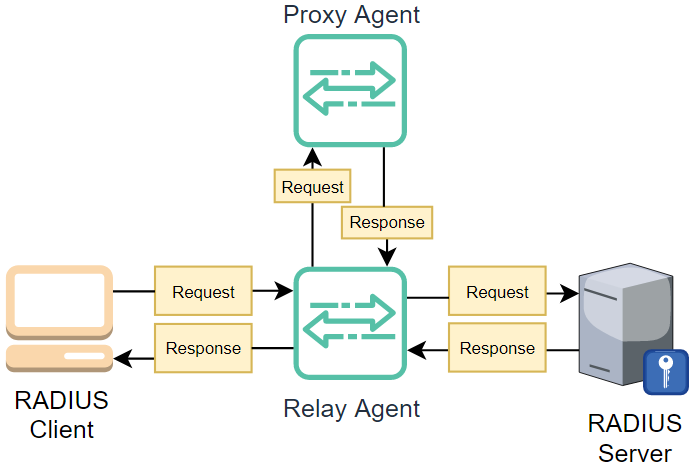
\includegraphics[width=0.8\textwidth]{image/relayagent.png}
    \caption{Relay Agent}
    \label{fig:relayagent}
\end{figure}